\section{Simulation}

In this section is presented the simulation of the design obtained from the previous section in Cadence.

The first step was to simulate the circuit with the transistors specifications obtained from the optimization process. Subsequently, was performed a fine-tuning of the circuit to improve the results by performing the value sweep of the most critical transistors.

The schematic of the circuit obtained in Cadence is shown in Figure \ref{fig:WL}. The final values of the transistors are shown in Table \ref{tab:WL}.

\begin{figure}[H]
    \centering
    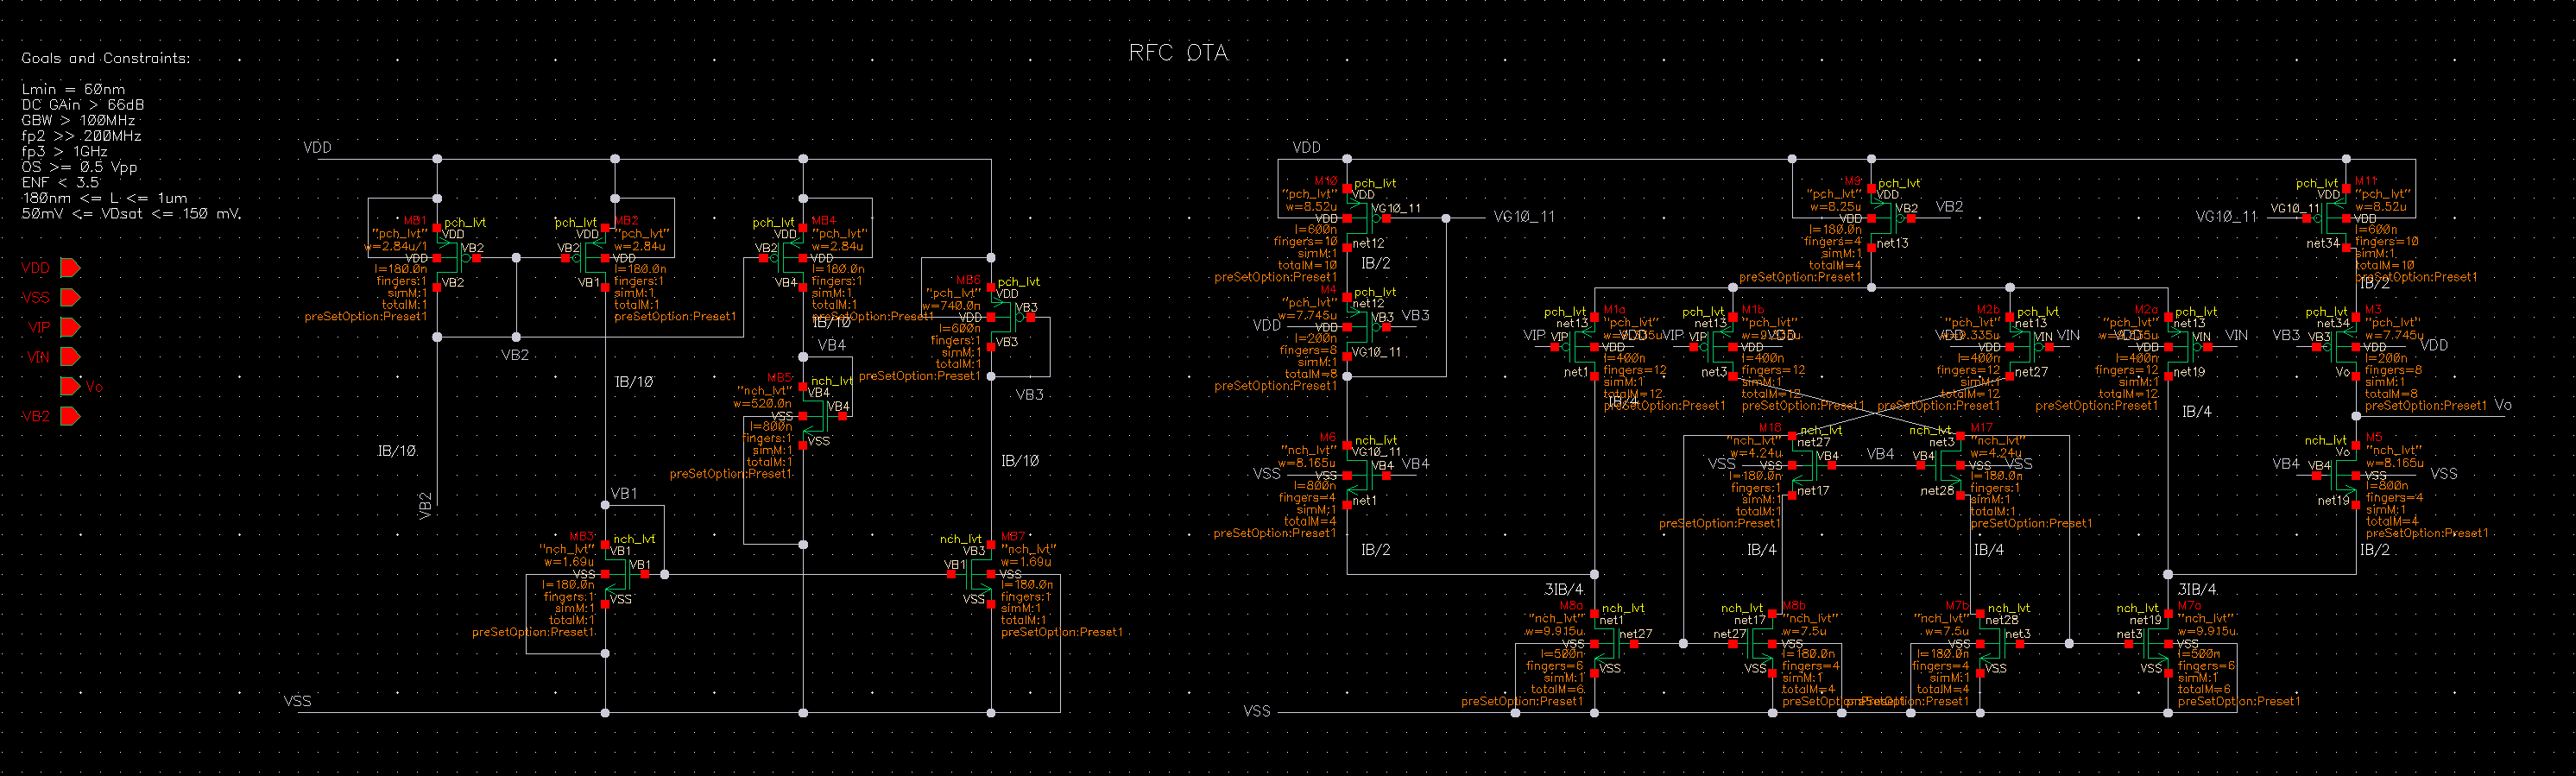
\includegraphics[width=1\textwidth]{Images/wLcircuit.png}
    \caption{Schematic of the circuit in Cadence.}
    \label{fig:WL}
\end{figure}

\begin{table}[h]
    \centering
    \caption{Transistors final dimensions}
    \begin{tabularx}{\textwidth}{>{\centering\arraybackslash}X >{\centering\arraybackslash}X >{\centering\arraybackslash}X}
        \toprule
        \textbf{Transistor} & \textbf{Length (L)} & \textbf{Width (W)}\\
        \midrule
        M1a & L & W\\
        \midrule
        M1a & L & W\\
        \bottomrule
    \end{tabularx}
    \label{tab:WL}
\end{table}


After the schematic was completed and verified, the symbol of the circuit was created to be used in the simulations. The testing circuit used for simulations is shown in Figure \ref{fig:Symbol}.

\begin{figure}[H]
    \centering
    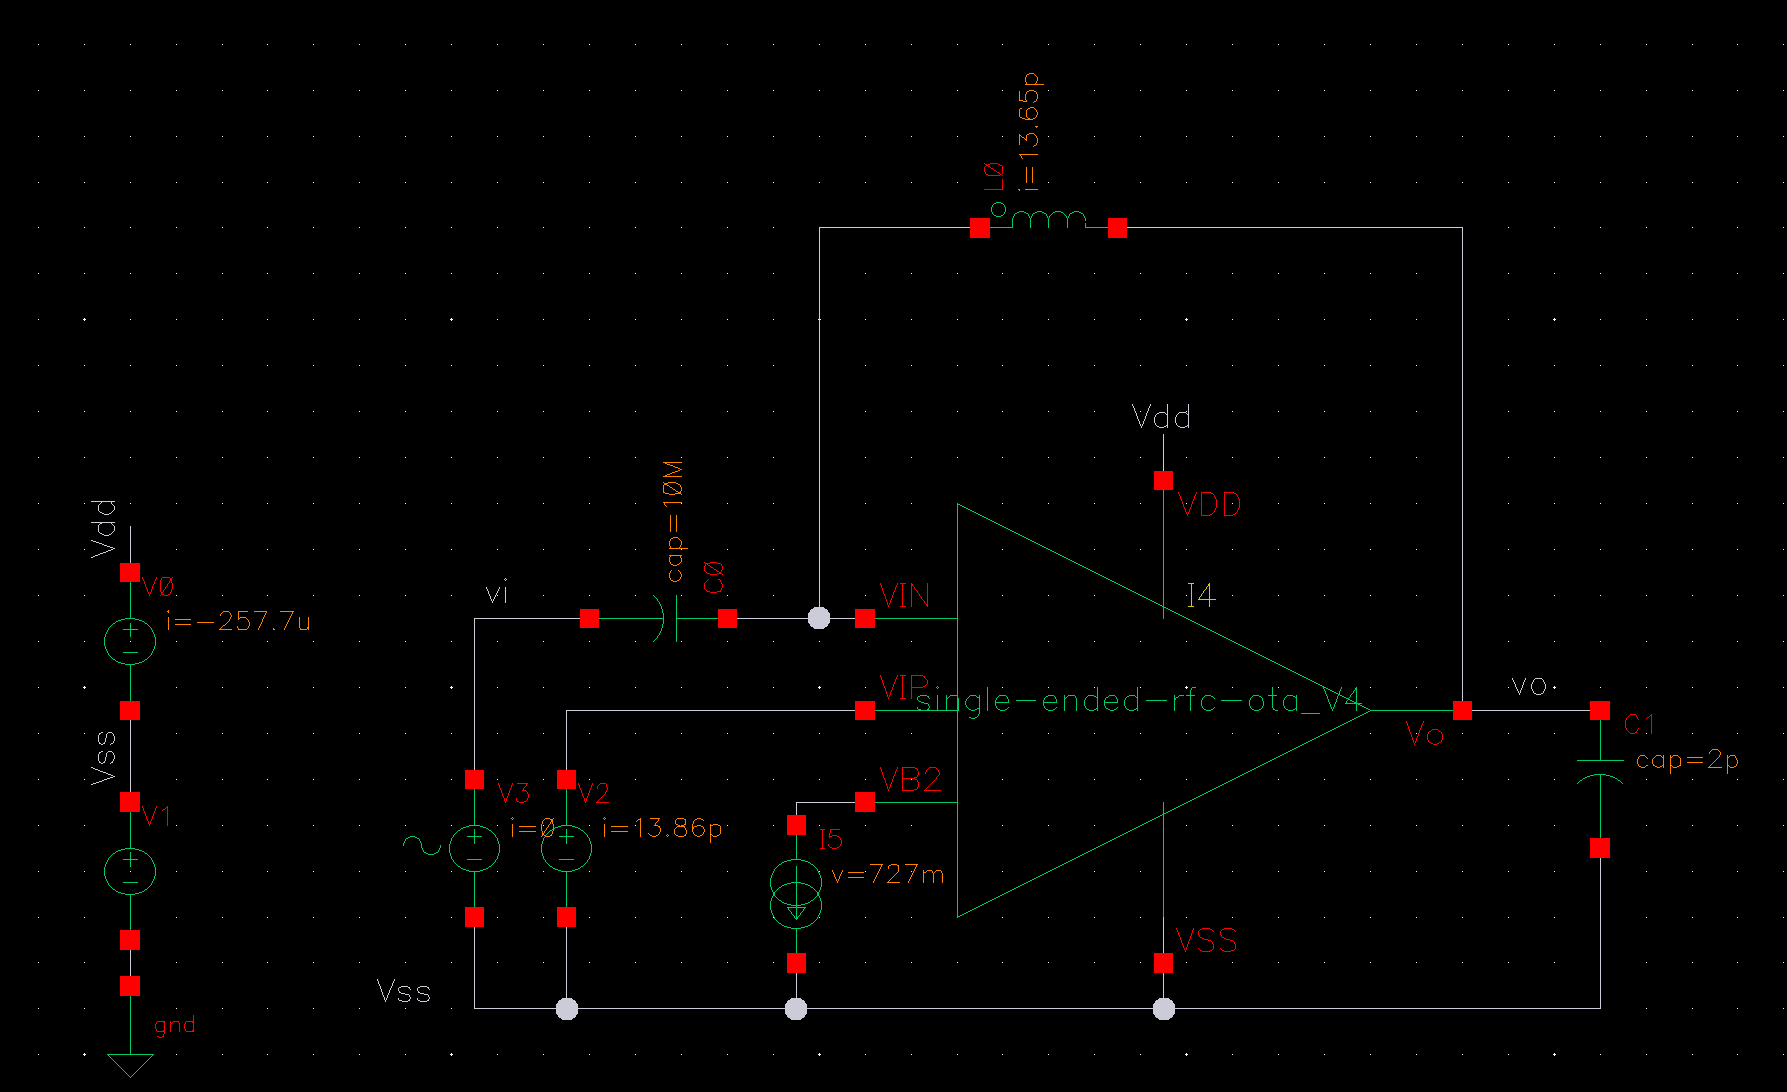
\includegraphics[width=0.5\textwidth]{Images/tb.png}
    \caption{Symbol of the circuit in Cadence.}
    \label{fig:Symbol}
\end{figure}

\subsection{DC Simulation}

The DC simulation was performed to verify the biasing of the circuit, in Figure \ref{fig:DC} is shown the results obtained.
The results were also compiled in Table \ref{tab:DC}.

\begin{figure}[H]
    \centering
    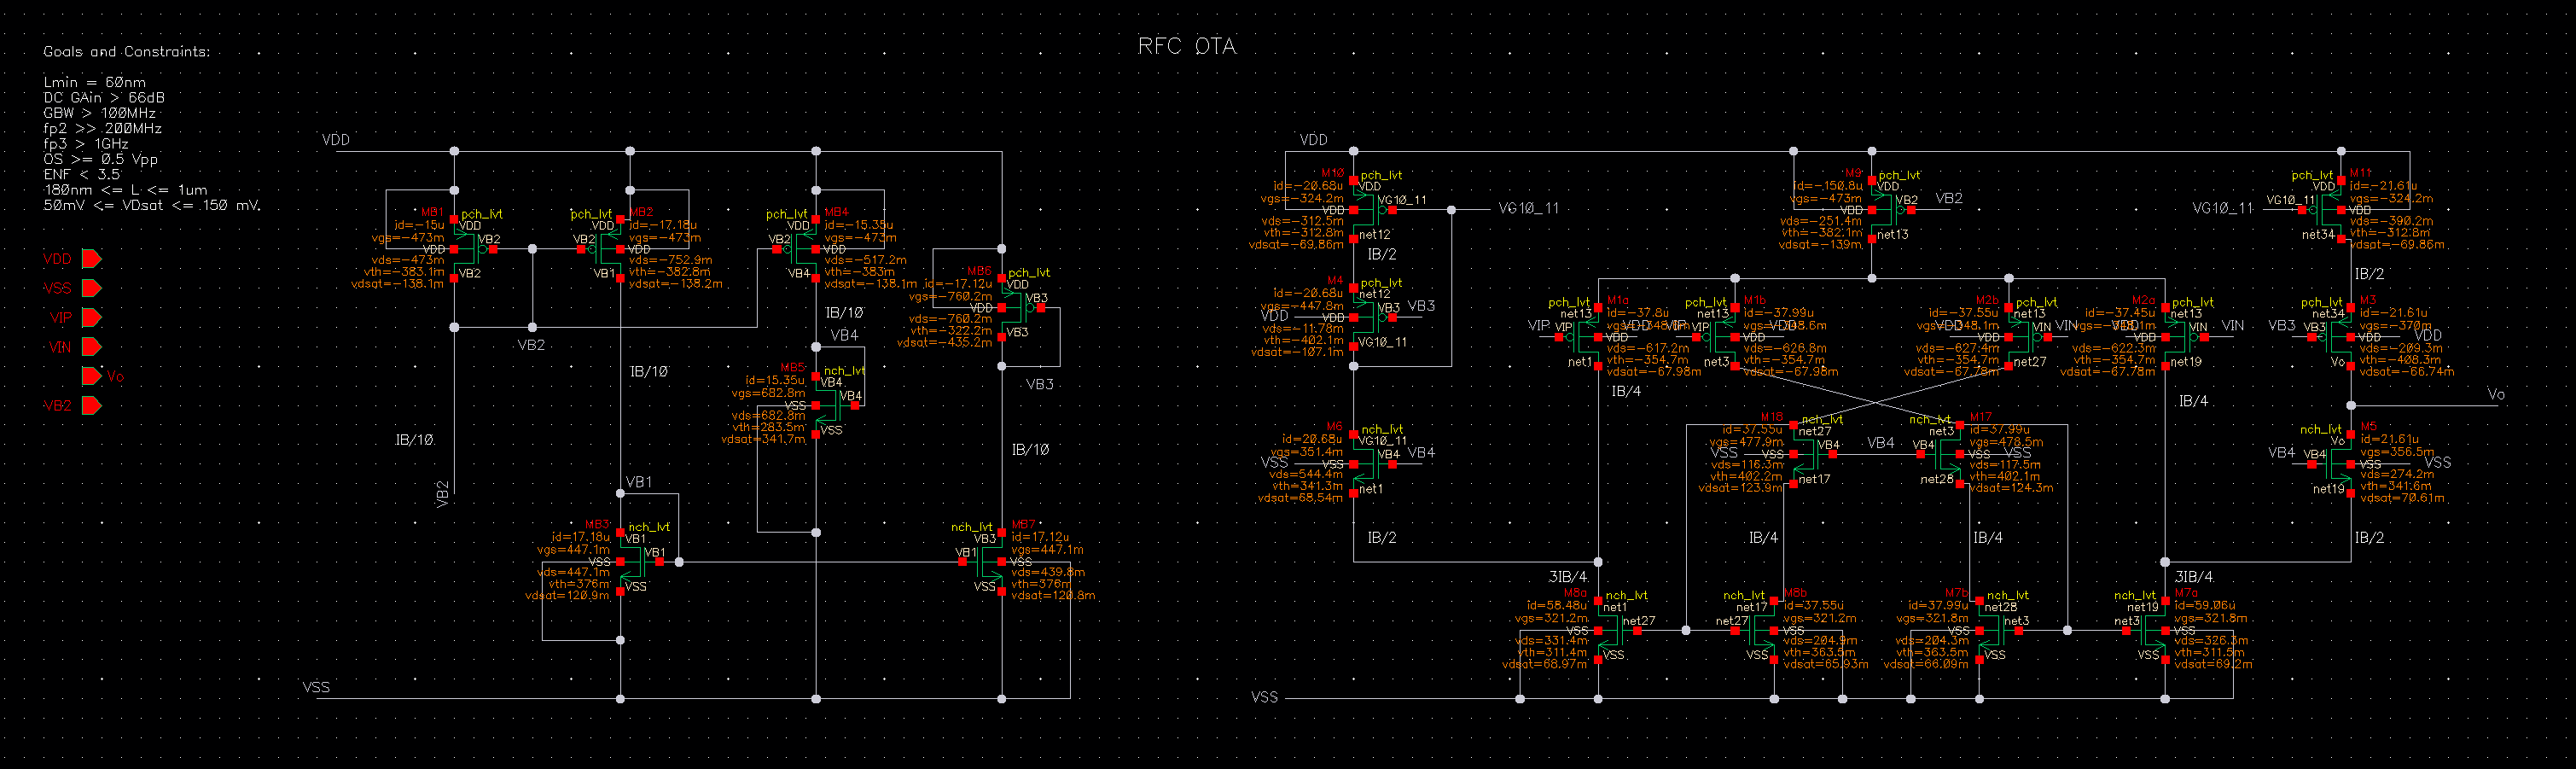
\includegraphics[width=1\textwidth]{Images/OP.png}
    \caption{Schematic of the circuit in Cadence}
    \label{fig:DC}
\end{figure}

\begin{table}[h]
    \centering
    \caption{DC simulation results}
    \begin{tabularx}{\textwidth}{>{\centering\arraybackslash}X >{\centering\arraybackslash}X >{\centering\arraybackslash}X}
        \toprule
        \textbf{Transistor} & \textbf{$V_{DSat}$} & \textbf{$I_B$}\\
        \midrule
        M1a & vdsat & Ib\\
        \midrule
        M1a & vdsat & Ib\\
        \bottomrule
    \end{tabularx}
    \label{tab:DC}
\end{table}

Observing the results obtained, it is possible to verify that the biasing of the circuit is correct, and the transistors are in the moderate inversion region.
\subsection{AC Simulation}

The AC simulation was performed to verify the gain and bandwidth of the circuit. The bode diagram obtained is shown in Figure \ref{fig:bode}.

\begin{figure}[H]
    \centering
    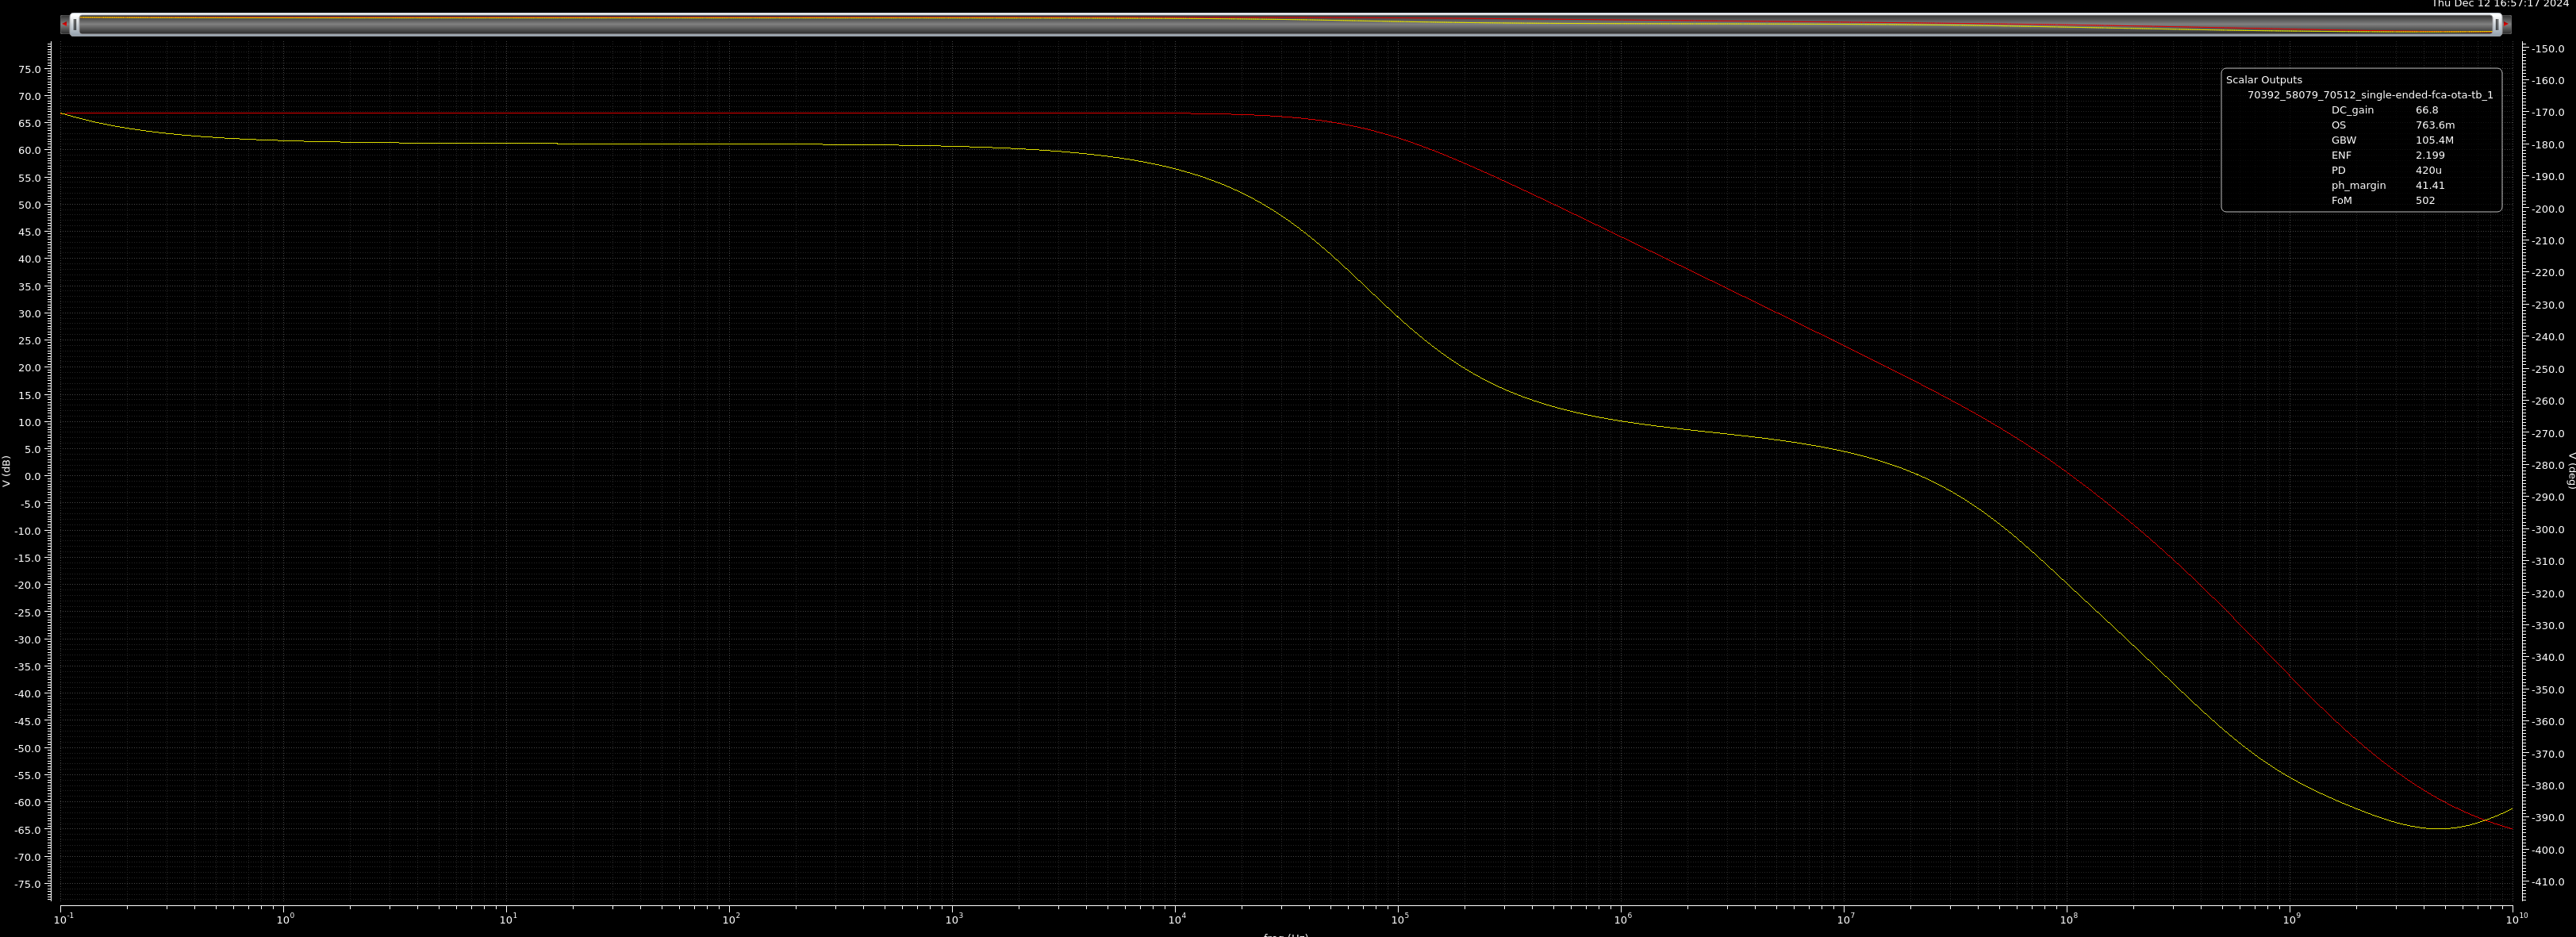
\includegraphics[width=1\textwidth]{Images/bode.png}
    \caption{Bode diagram of the circuit.}
    \label{fig:bode}
\end{figure}

The results obtained are shown in Table \ref{tab:AC}.

\begin{table}[h]
    \centering
    \caption{AC simulation results}
    \begin{tabularx}{\textwidth}{>{\centering\arraybackslash}X >{\centering\arraybackslash}X }
        \toprule
        \textbf{Parameter} & \textbf{Result} \\
        \midrule
        DC Gain & \SI{66.8}{\decibel} \\
        \midrule
        Gain Bandwidth Product & \SI{105.4}{\mega\hertz}\\
        \midrule
        Phase Margin & \SI{41.41}{\degree}\\
        \midrule
        Output Swing & \SI{763.6}{\milli\volt}\\
        \midrule
        Power Dissipation & \SI{420}{\micro\watt}\\
        \midrule
        Excess-Noise Factor & 2.199 \\
        \midrule
        Figure of Merit & \SI{502}{\mega \hertz \cdot \pico \farad  / \milli \watt}\\
        \bottomrule
    \end{tabularx}
    \label{tab:AC}
\end{table}

\subsection{Layout}

A simplified layout of the circuit was performed to verify the area occupied by the circuit. The layout obtained is shown in Figure \ref{fig:layout}.

\begin{figure}[H]
    \centering
    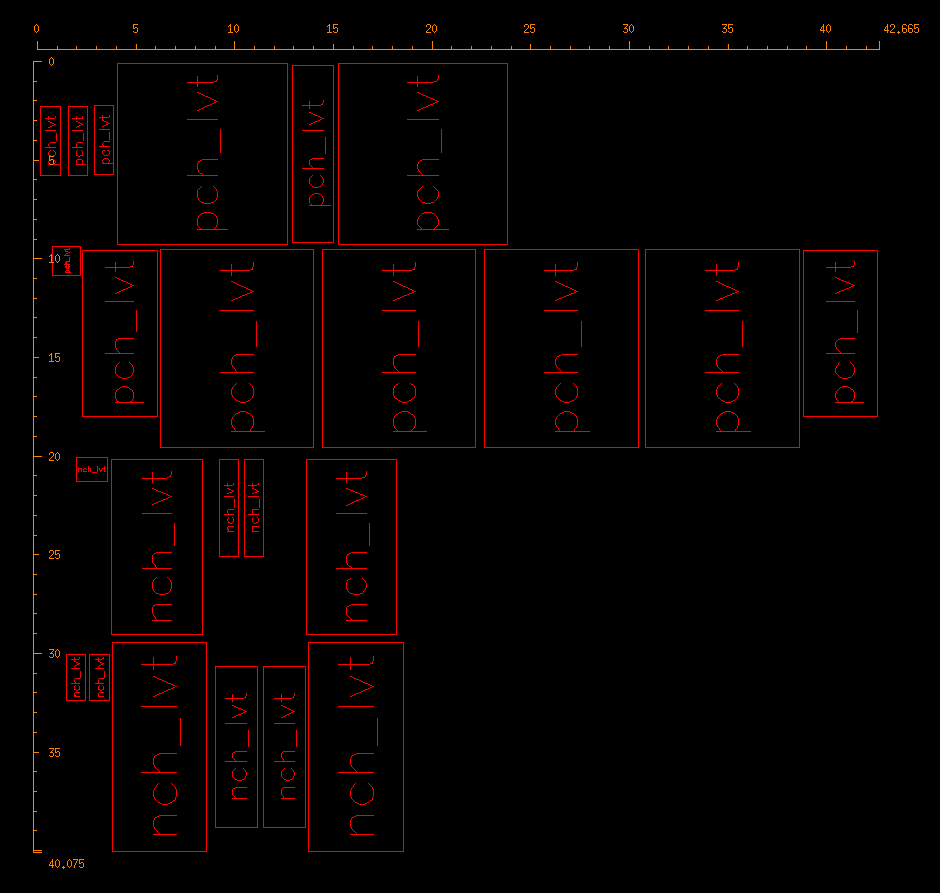
\includegraphics[width=0.6\textwidth]{Images/layout.png}
    \caption{Simplified layout of the circuit.}
    \label{fig:layout}
\end{figure}